\chapter{Weitere Entwicklungen}\label{cha:Weitere Entwicklungen}

Nachdem die Grundlegende Plattform für das Projekt zu Verfügung steht befinden sich eine Reihe weiterer Verbesserungen und Innovationen in Arbeit. Diese sollen sowohl das Elektroniksystem bezüglich Handhabung, Sicherheit und Leistung optimieren, als auch neue Aspekte welche bisher keine genaue Beachtung erfahren haben, mit Angepassten Technischen Lösungen versehen.


\section{Entwicklung weiterer Funktionen als Modul}

Das Konzept des fertig aufgebauten,erprobten und bevorrateten Moduls der Idealen Diode als auflötbaren klein PCB hat sich bewährt. Eine Reihe von Anwendungen auch außerhalb der Flugzeugelektronik haben die Zeitersparniss bei der Entwicklung gezeigt und eine zuverlässige Funktion gewährleistet.
Deshalb sollen weitere Systemfunktionen als Modul realisiert werden.
Eine interissante Gruppe der Sensoren sind hier beispielsweise die Analog Digital Wandler (ADC). Während die Implementierung des einzelnen ADC in Hardware und Software aufwendig ist, ermöglicht die Anbindung an den I2C Bus den Einsatz vieler gleicher Messplatinen Beispielsweise zur Überwachung der einzelnen Akkuspannungen.
Auch bisher nicht realisierte Konzepte wie die Rückführung der Realen Ruderwinkel über Encoder oder Hall Sensoren sind in der Kombination aus PCB Modul und CAN Bus realisierbar.

Insgesamt bietet sich das Modulkonzept bei allen Elektrischen Bauteilen an bei denen ein hoher Aufwand für Auslegung, Layout und Erprobung betrieben werden muss um eine zuverlässige Funktion sicherzustellen.

\section{Betrachtung des CAN Bus}

Während in der manntragenden Luftfahrt der CAN Bus bereits seit langem zum Standard zur Übertragung von Sensordaten und auch Steuersignalen eingesetzt wird wurde er bisher im bereich kleiner UAV System kaum verwendet. Hauptgrund dafür stellt die strukturelle  Komplexität des vollständig Paket basierten Datenbusses dar, sowie die Softwareseitig aufwendige Adressierung und Verwaltung der einzelnen Teilnehmer.
Mit dem erscheinen des Pixhawk 2 wird der CAN Bus als regulärer Systembus geführt und seine Softwarepakte von der Offiziellen Entwicklergruppe gepflegt. Damit entfällt in Anbetracht der berenzten Personal Ressourcen im Labor der bisher Aufwendigste Aspekt der Nutzung dieses Systems. Eine Nutzung der hohen Stabilität bei geringer Leitungszahl und aber auch Flexibilität bei der Anzahl der Teilnehmer wird damit als Sensorbus möglich.
Entsprechend CAN Bus fähige Sensorplatinen sollen als Module konzeptioniert werden.

\section{Schnellwechsel-Akkusystem aus Rundzellen}

Neben den bisher eingesetzten Akku Packs aus Folienzellen stehen am Markt eine große Bandbreite and Rundzellen verschiedener Formate zur Verfügung. Als Industrielle Massenware stellen sie sich unter anderem als Preisgünstige Alternative dar.
Eine Analyse des Energie zu Gewicht Verhältnis ergab einen deutlich besseren Wert für die einzelnen Rundzellen gegenüber den Vorliegenden Folienzellen.Erste Prototypen eines Modularen Akkupakets aus 18650 Lithium Polymer Rundzellen der Firma LG lassen eine Verbesserung des Kwh/kg Wertes um 15 bis 25 Prozent erwarten.
Außerdem soll der neue Packaufbau die Handhabung Verbessern indem der Akku Tausch Ohne eine Demontage des Flügels möglich ist.Zur weiteren Vereinfachung soll auch das in den Röhrenförmige Paketaufbau integrierte Anschlussstecksystem beitragen.

Eine Erprobung der nötigen Verbindungstechniken und die Konstruktion eines Entsprechenden Gesamtpaketes findet derzeit statt.
Im weiteren Verlauf soll noch die genaue Integration in den Flügel und das gesamte Elektroniksystem gelöst werden.

\begin{figure}[H]
\centering
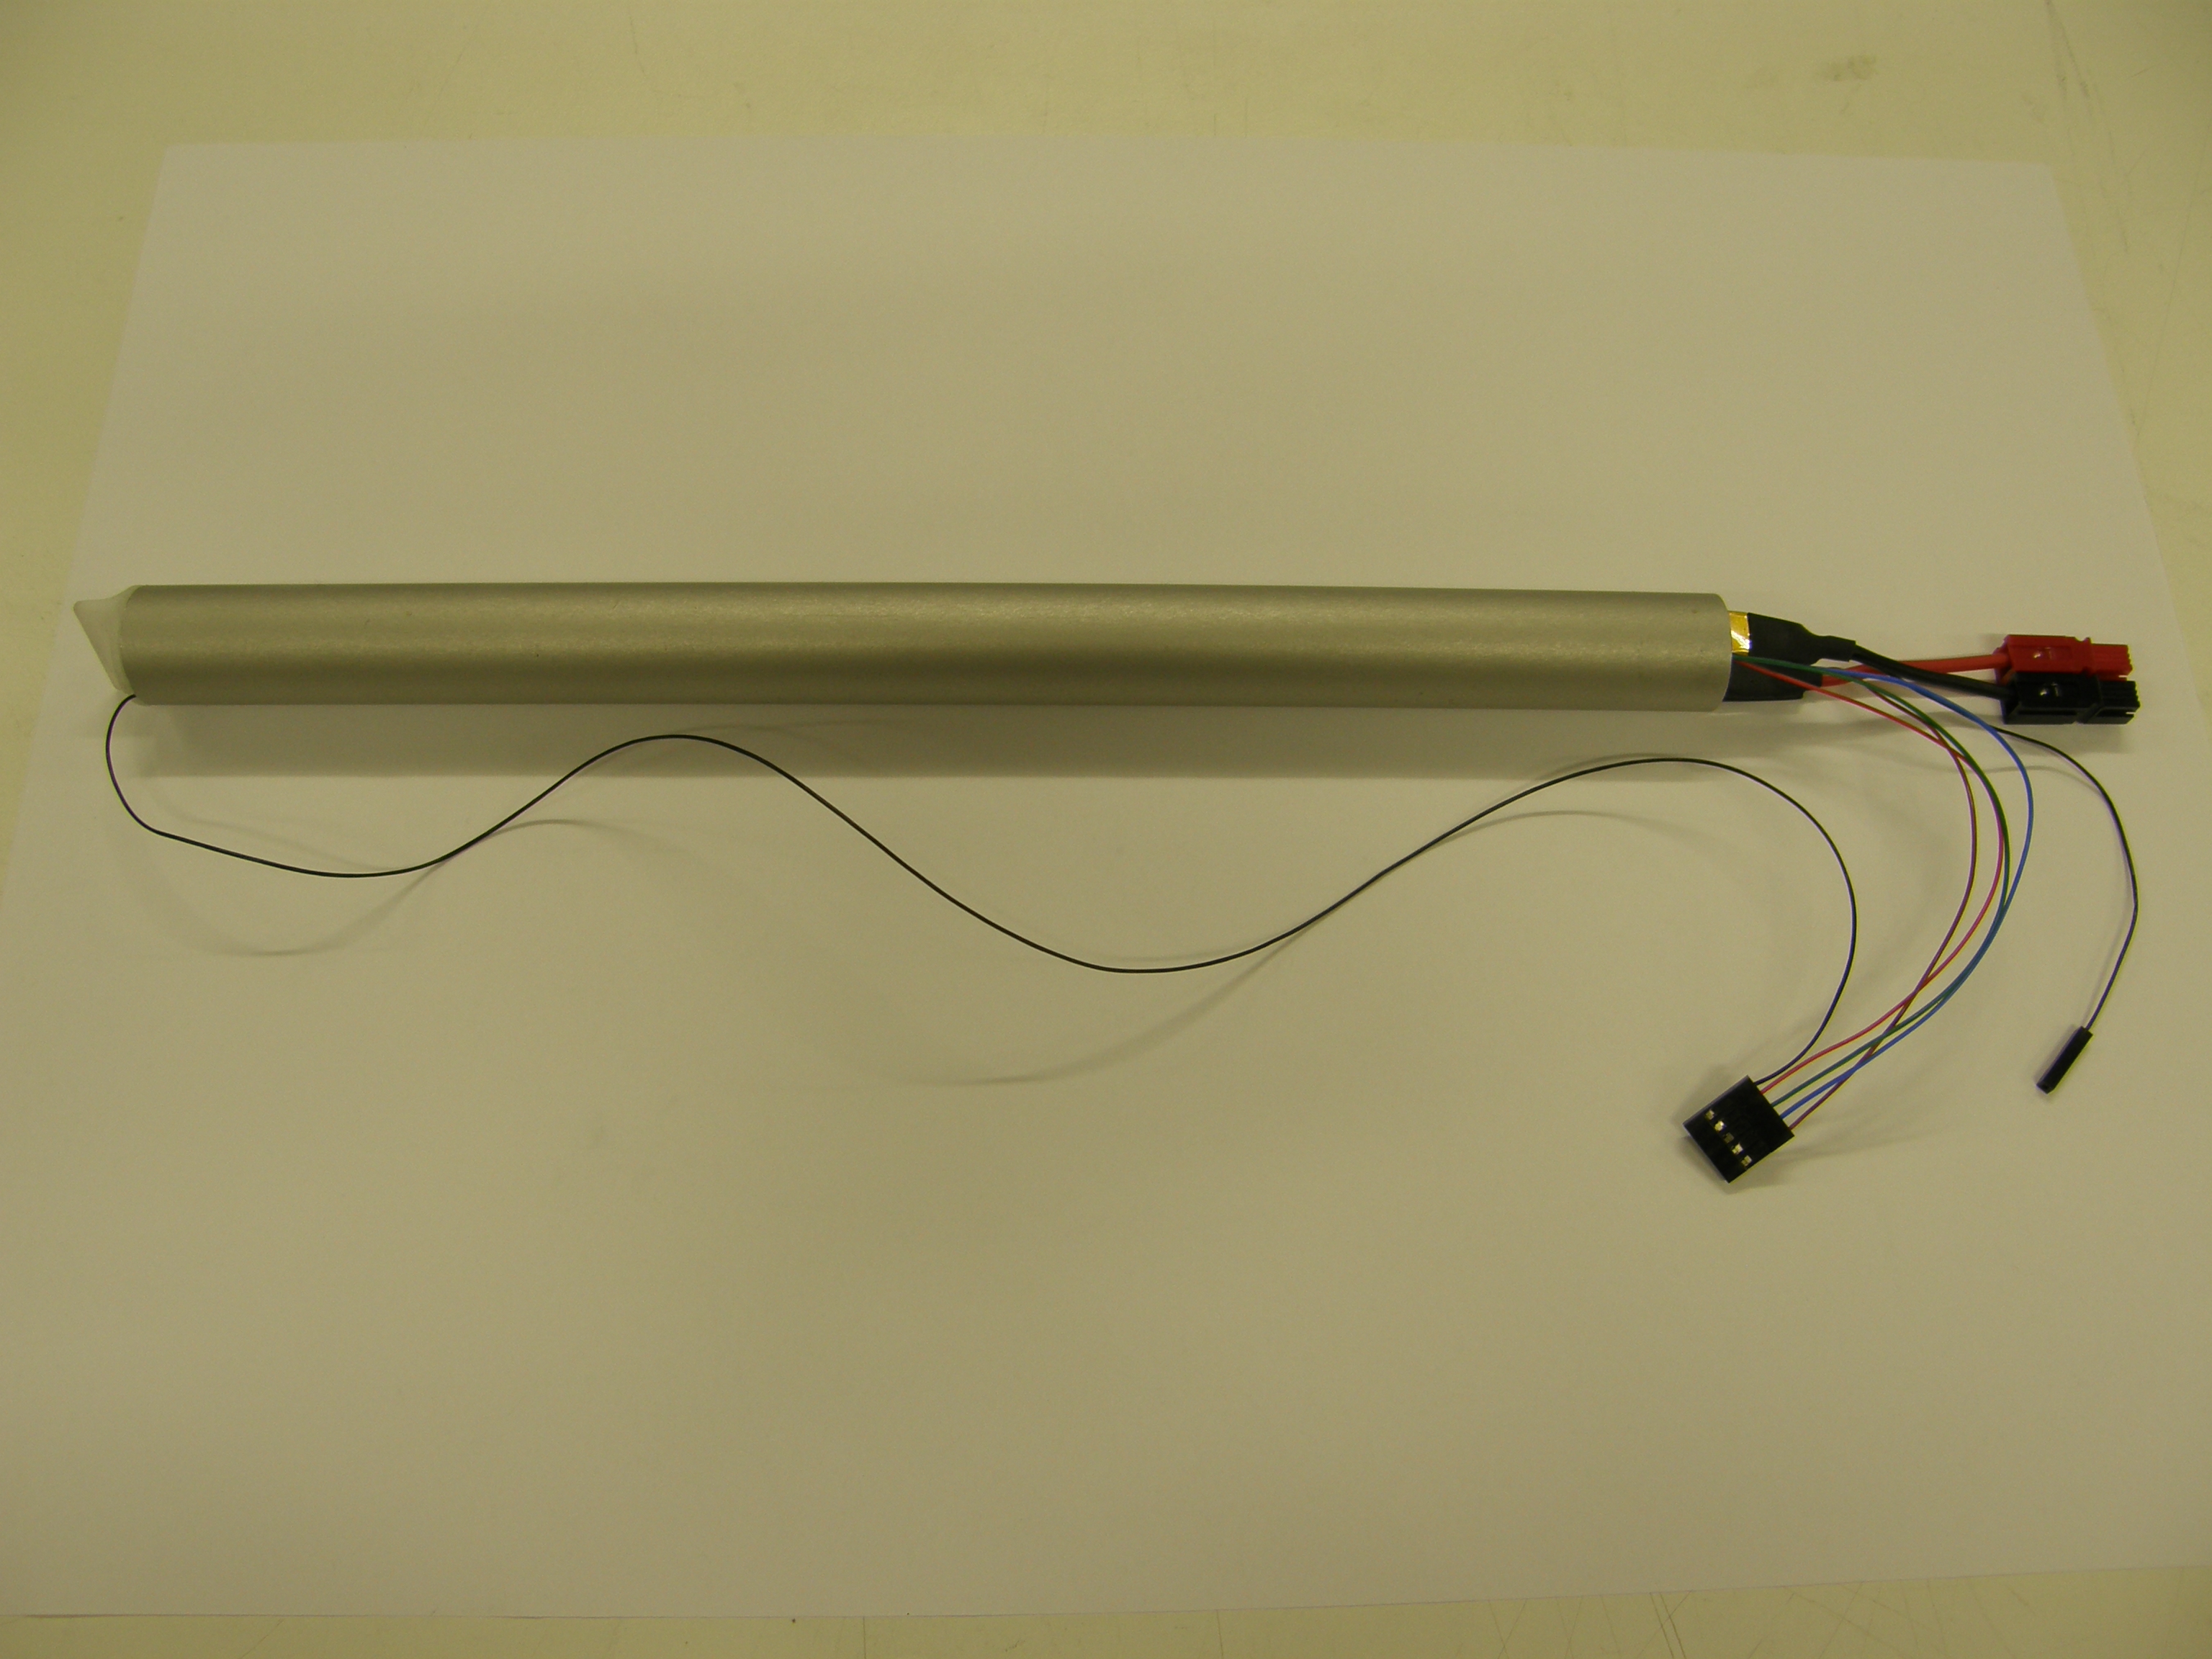
\includegraphics[width=0.9\textwidth]{bilder/Fotos/Prototyp_18650er_Zellensystem.jpg} 
\caption{Zweiter Prototyp der Runzellenpakets} 
\label{fig:Zweiter Prototyp der Runzellenpakets}
\end{figure}

\section{Migration auf die nächste Pixhawk Generation}

Im Zuge des Wachstums des Pixhawk Projekts wurde eine neue Generation von Hardware für den ArduPilot Autopiloten entworfen und in den Software branch eingepflegt. Diese leistungsgesteigerte Version steht seit Anfang 2017 zu Verfügung.
Sie verfügt neben mehr Prozessorleistung und rendundanten integrierten Sensoren über eine DF17 80 Pin Schnittstelle der Firma JST. Damit ist eine noch Platzsparendere Unterbringung des Pixhawk möglich und es werden weitere Kabelverbindungen eingespart.

Um diese Komponente in Zukunft im Flugsystem nutzen zu können, wird eine Entsprechende Platinenentwicklung und die Nötige Integration seit Sommer 2017 von Michael Simbürger durchgeführt.

\begin{figure}[H]
\centering
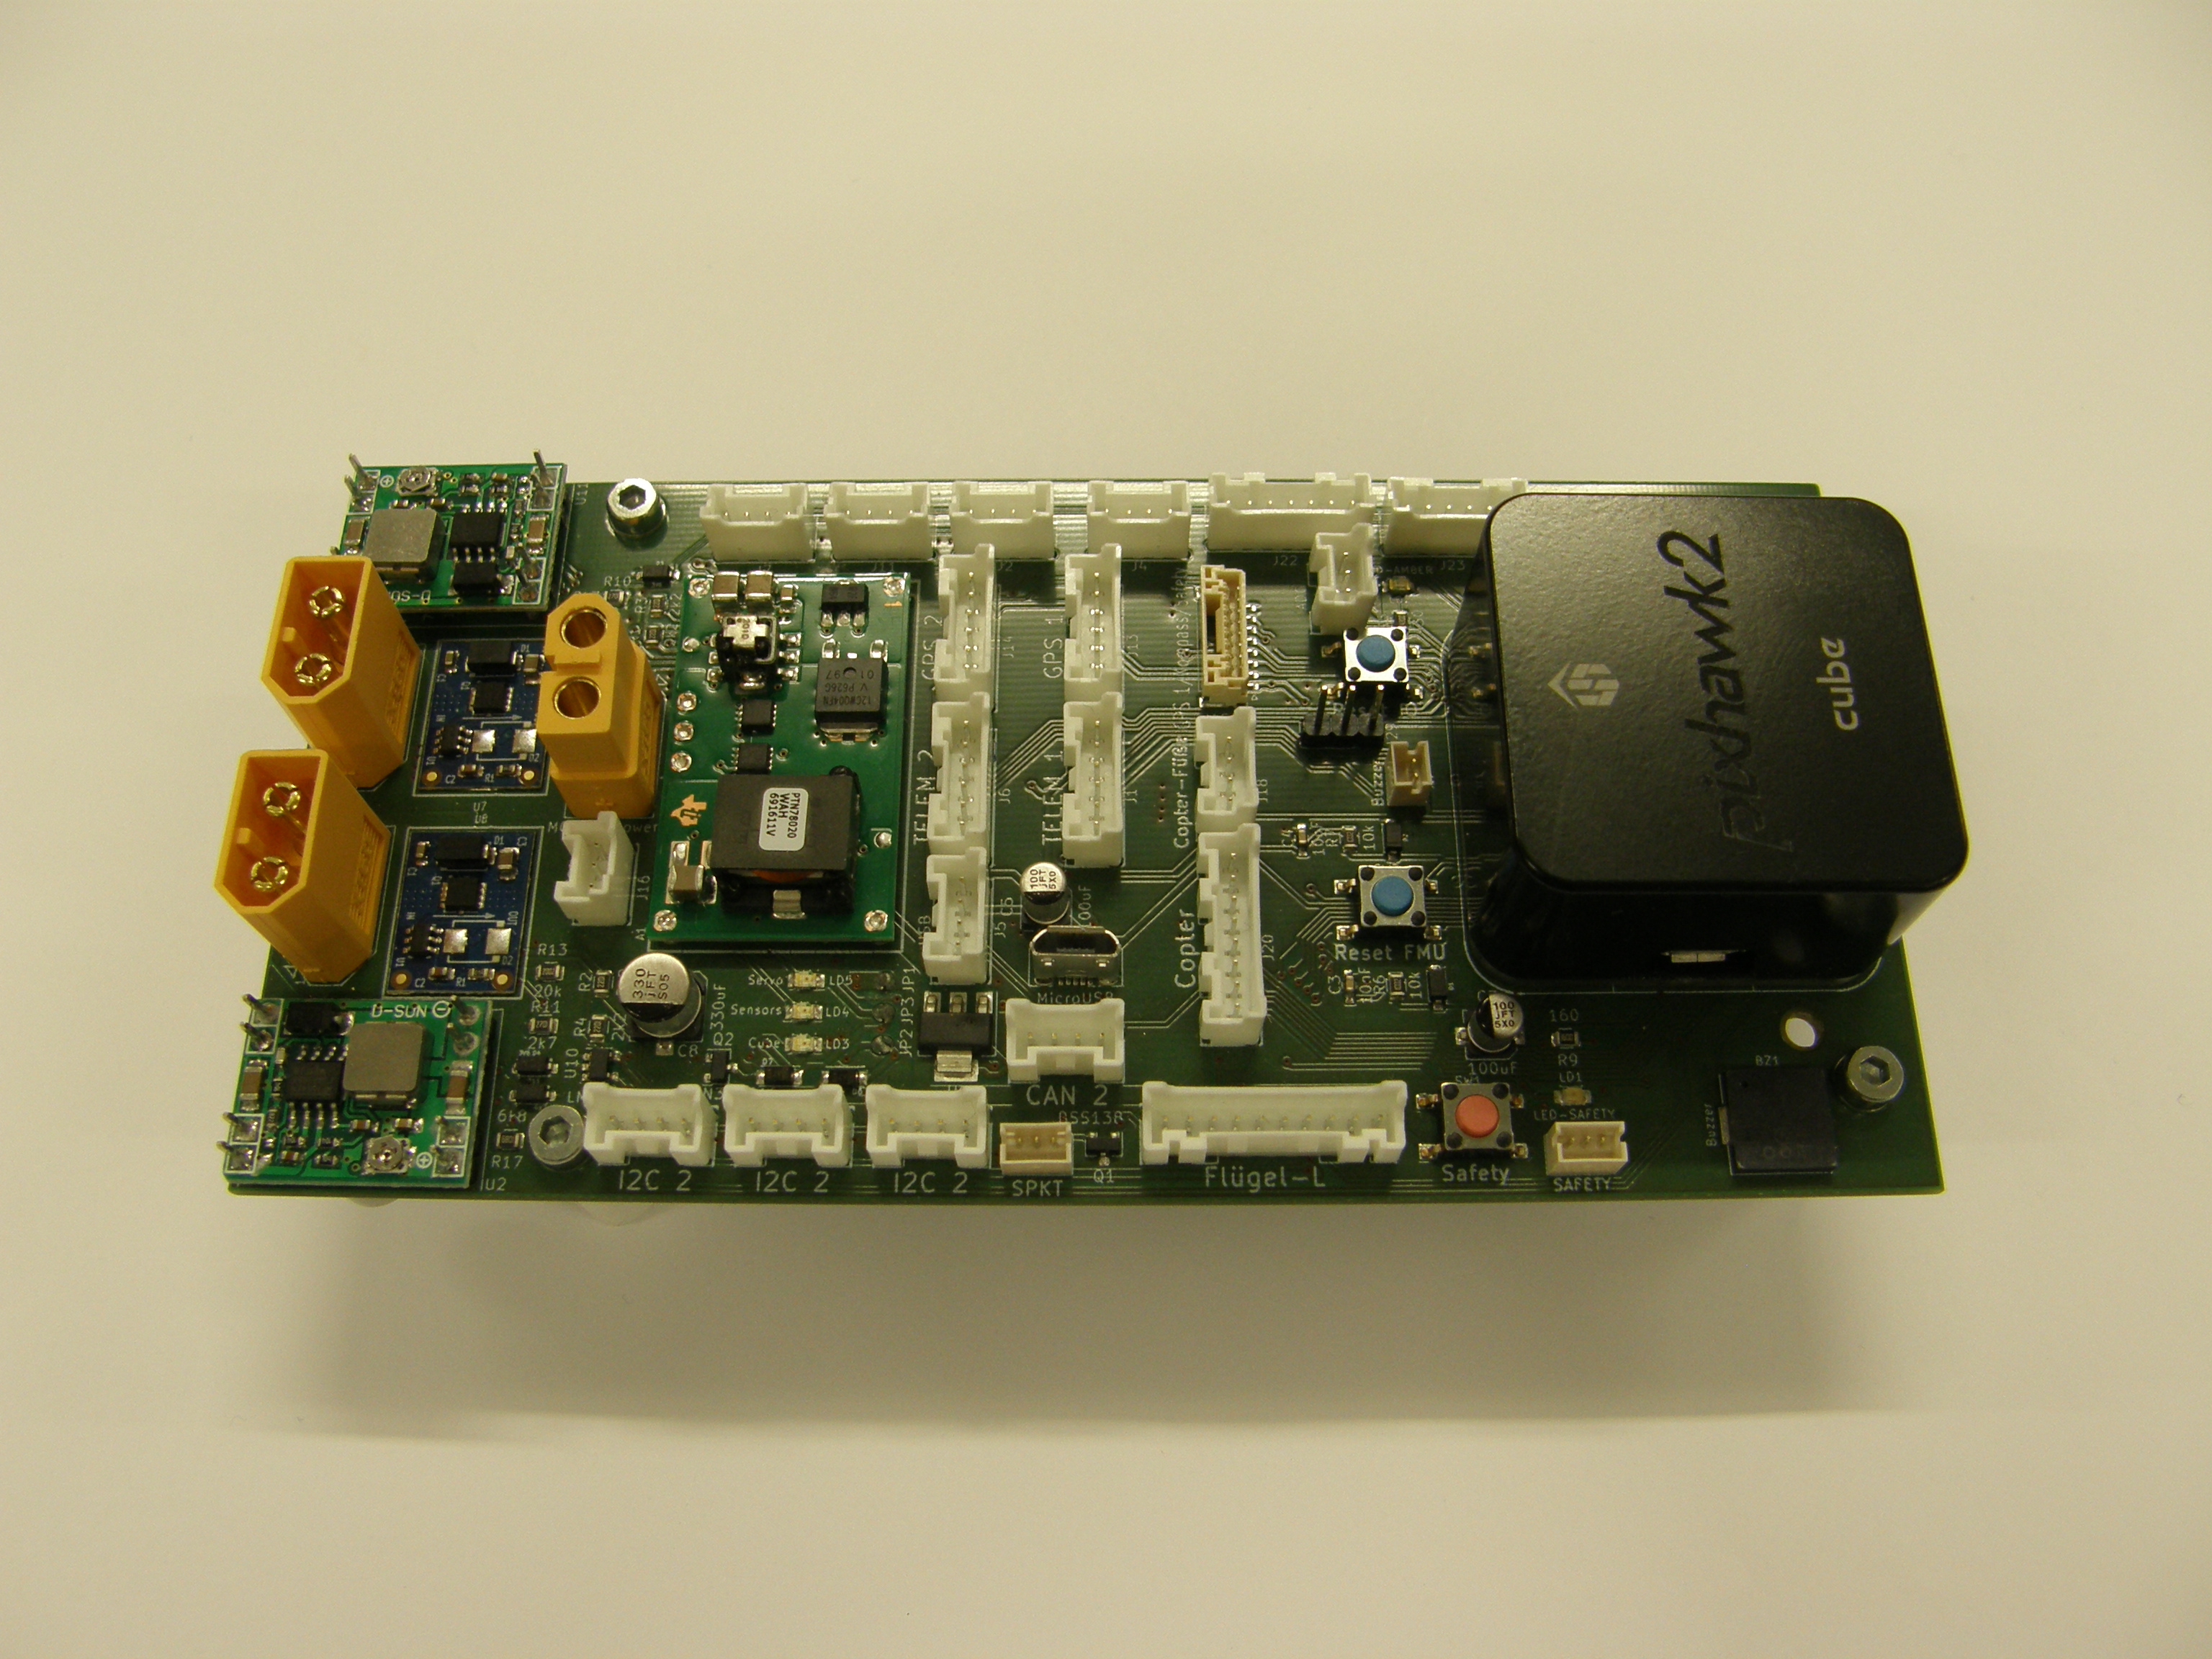
\includegraphics[width=0.9\textwidth]{bilder/Fotos/Pixhawk2_Autopilot_PCB_2018_Simbuerger.jpg} 
\caption{Neue Pixhawk 2 Autopilotenplatine für 2018 von Michael Simbürger} 
\label{fig:Neue Pixhawk 2 Autopilotenplatine für 2018 von Michael Simbürger}
\end{figure}

%\section{Erfahrungen aus dem Feldeinsatz}

%\section{Anpassung der Anforderungen an die Elektronik}

%\section{Detailverbesserungen an den Komponenten}

%\section{Technischer Ausblick}